Nền tảng kỹ thuật đầu tiên của CausClass là phát hiện hành vi trong từng khung hình video. Những năm gần đây, phát hiện đối tượng thời gian thực phát triển mạnh nhờ các mạng nơ-ron sâu và các biến thể của YOLO. YOLO thực hiện định vị và phân loại trong một lần suy luận, nhờ đó phù hợp với các ứng dụng cần xử lý video nhanh \,\cite{redmon2016yolo}. Các thế hệ sau như YOLOv7, YOLOv9 và YOLOv10 tiếp tục cải thiện hiệu năng thông qua thiết kế kiến trúc, kỹ thuật huấn luyện và tối ưu suy luận \,\cite{wang2023yolov7,wang2024yolov9,wang2024yolov10}. Song song với nhánh YOLO, các detector dựa trên transformer như RT-DETR cũng cho thấy hướng thiết kế end-to-end thời gian thực là một xu thế quan trọng trong phát hiện đối tượng hiện đại \,\cite{zhao2024rtdetr}.

YOLO26 là thế hệ mới hơn trong hệ sinh thái Ultralytics, được thiết kế như một họ mô hình thị giác thời gian thực thống nhất cho nhiều tác vụ như phát hiện đối tượng, phân đoạn, ước lượng tư thế, phân loại và phát hiện hộp xoay \,\cite{jocher2026ultralyticsyolo26unifiedrealtime}. Về phát hiện đối tượng, YOLO26 sử dụng thiết kế hai head để hỗ trợ suy luận end-to-end không cần NMS ở đường mặc định, đồng thời làm nhẹ head hồi quy hộp. Họ mô hình gồm nhiều thang kích thước \(n/s/m/l/x\); trong đó YOLO26n là biến thể nhỏ, phù hợp làm detector nền cho pipeline video cần xử lý nhiều khung hình.

Trong bối cảnh lớp học, phát hiện hành vi khó hơn phát hiện đối tượng thông thường vì nhãn hành vi thường phụ thuộc vào ngữ cảnh. Đọc và viết đều liên quan đến tư thế ngồi; cúi đầu có thể giống đọc sách; sử dụng điện thoại có thể bị che bởi tay, bàn hoặc vở. Các tín hiệu quan trọng có thể nằm ở nhiều vùng ảnh khác nhau như đầu, tay, bàn học, sách vở và vật thể nhỏ. Vì vậy, detector cần không chỉ nhận dạng đặc trưng cục bộ mà còn cần tổng hợp quan hệ không gian xa.

Cơ chế attention cung cấp một cách bổ sung ngữ cảnh cho detector. Khác với tích chập, vốn chủ yếu tổng hợp thông tin trong vùng lân cận, self-attention cho phép các vị trí ảnh trao đổi thông tin trên phạm vi rộng và kế thừa trực tiếp ý tưởng attention đa đầu trong kiến trúc Transformer \,\cite{vaswani2017attention}. Tuy nhiên, self-attention toàn cục trên ảnh độ phân giải cao có chi phí lớn, nên nhiều nghiên cứu tập trung vào attention hiệu quả cho tác vụ thị giác dày đặc. EfficientViT dùng attention tuyến tính đa tỉ lệ để giảm độ phức tạp \,\cite{cai2023efficientvit}, còn BiFormer dùng bi-level routing attention để phân bổ tính toán cho các vùng ảnh giàu thông tin hơn \,\cite{zhu2023biformer}.

Trong đồ án này, Multi-Head Self-Attention được dùng như một khối bổ sung cục bộ trong YOLO26n-MHSA. Mục tiêu không phải thay thế toàn bộ detector bằng transformer, mà là kiểm tra xem một lượng attention hạn chế trong đường tổng hợp đặc trưng có giúp mô hình hóa quan hệ giữa các vùng ảnh quan trọng hay không. Cách thiết kế này giữ phần lớn kiến trúc YOLO26n để so sánh với baseline rõ ràng hơn, đồng thời vẫn đưa vào khả năng nắm bắt phụ thuộc không gian xa.

Hình~\ref{fig:yolov8-mhsa-detection} minh họa kết quả phát hiện hành vi lớp học trong một nghiên cứu dùng YOLOv8 kết hợp cơ chế attention. Ví dụ này cho thấy attention có thể hỗ trợ detector trong bối cảnh nhiều học sinh và nhiều vùng ảnh liên quan đến cùng một hành vi.

\begin{figure}[H]
  \centering
  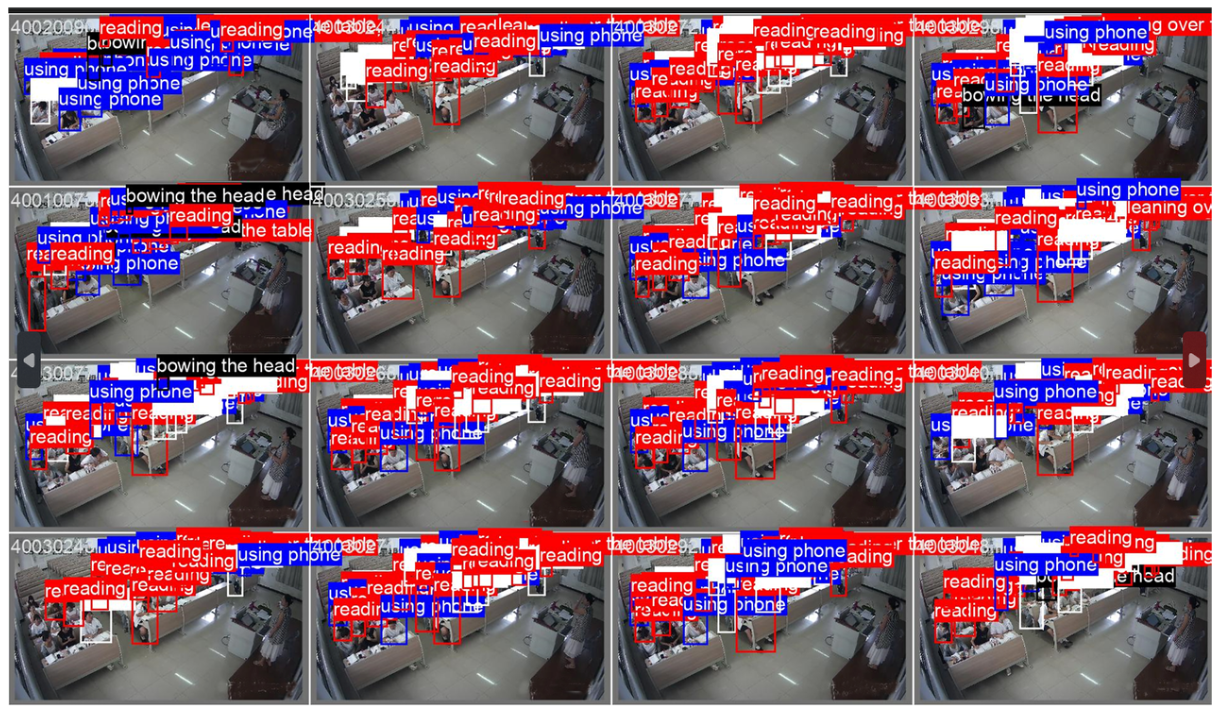
\includegraphics[width=0.9\textwidth]{figures/yolov8.png}
  \caption{Minh họa kết quả phát hiện hành vi lớp học bằng YOLOv8 kết hợp cơ chế attention. Nguồn: Zhang và cộng sự \cite{zhang2025yolov8attention}.}
  \label{fig:yolov8-mhsa-detection}
\end{figure}

Sau khi phát hiện theo khung hình, hệ thống cần duy trì sự liên tục của đối tượng qua thời gian. ByteTrack là một phương pháp multi-object tracking liên kết các hộp phát hiện thành track bằng cách tận dụng cả hộp điểm cao và hộp điểm thấp \,\cite{zhang2022bytetrack}. Trong CausClass, ByteTrack giúp biến các phát hiện rời rạc thành các đoạn sự kiện có thời gian bắt đầu--kết thúc, tạo đầu vào ổn định hơn cho bước gom time bin.
